\section{Results and Discussion}
Depending on your topic you may wish to separate this into two sections.

Here you will need to include figures and tables. Please reference the figures in the text like this: The \textbf{Figure \ref{map_struct}} demonstrates a schematic overview of MAP Programme Structure. Subsequent references to the same figure can be abbreviated and should not be in bold (i.e. Fig. \ref{map_struct}).

\begin{figure}
	\centering
	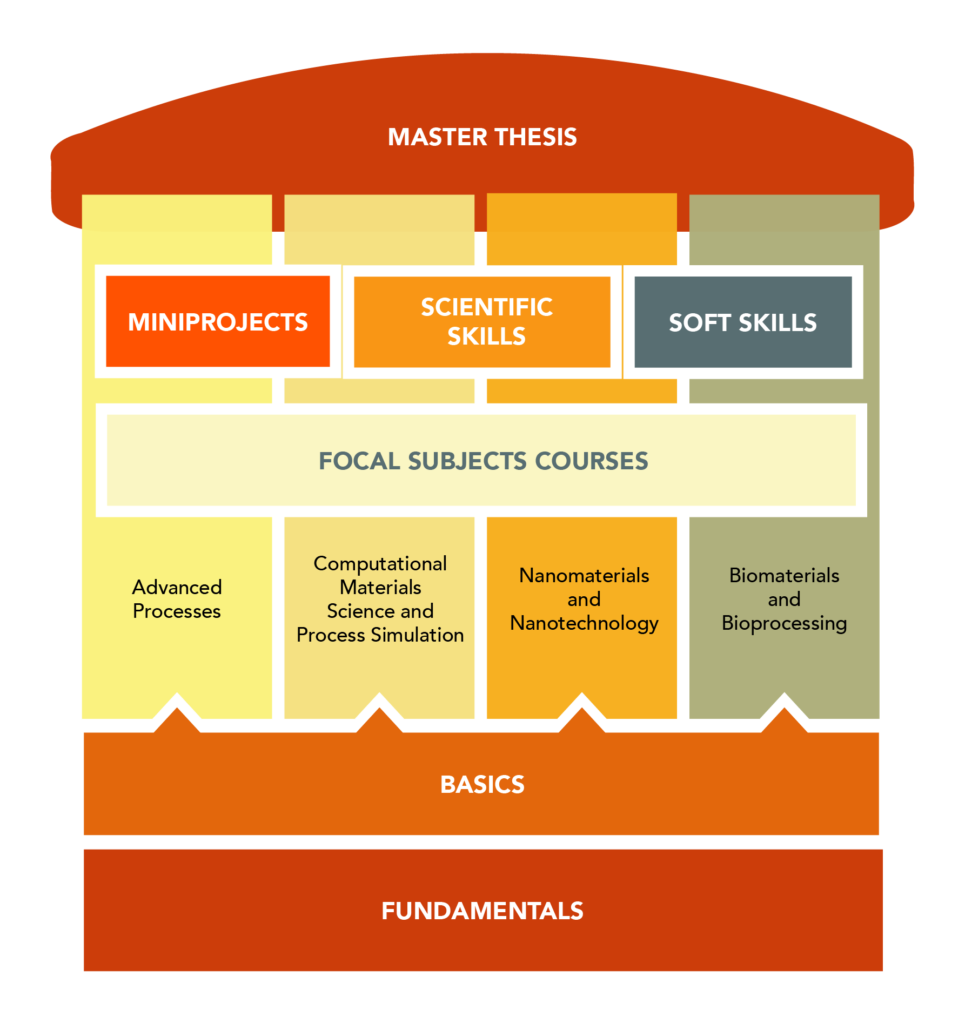
\includegraphics[width=0.5\textwidth]{map_structure}
	\caption{MAP program structure\cite{map_web}}
	\label{map_struct}
\end{figure}

Tables should be referenced in the same way as figures (though “Table” should always be written out in full). The table caption should be placed above the table.
 
To use pictures in \LaTeX \ you should first save your images to the folder \textit{images/}. If you want to use other directories, specify them in the \textit{main.tex} file in the \textbackslash graphicspath\{...\}.
 
You can easily create images and graphs with tikz. For example if you have the experimental data points don't hurry to create excel diagrams. Check out how the package pgfplots can be used to retrieve the data from csv files.